\documentclass[sigconf]{acmart}

\usepackage{booktabs} % For formal tables
\usepackage[inline]{enumitem}

%% \name command
%% - allows break before /
\usepackage{etoolbox}
\usepackage{xstring}
\DeclareListParser{\doslashlist}{/}
\newcounter{ndnNameComponentCounter}%
\newcommand{\name}[1]{{%
  \setcounter{ndnNameComponentCounter}{0}%
  \renewcommand{\do}[1]{{%
    \ifnumgreater{\value{ndnNameComponentCounter}}{0}{\allowbreak/}{}%
    \ifnumodd{\value{ndnNameComponentCounter}}{}{}%
    \detokenize{##1}}%
    \stepcounter{ndnNameComponentCounter}}%
``{\fontfamily{cmtt}\small\selectfont\IfBeginWith{#1}{/}{/}{}\doslashlist{#1}}''%
}}

\newcommand{\TODO}[1]{\textcolor{red}{#1}}

\begin{document}
\title{NDN IoT Protocols on RIOT OS}
%% LZ: this title sounds a bit too big, how aobut
%% a framework for home IoT networking over NDN?

\author{Tianyuan Yu}
\affiliation{%
	\institution{Sichuan University}
}
\email{royu9710@outlook.com}

\author{Zhiyi Zhang}
\affiliation{%
  \institution{UCLA}
}
\email{zhiyi@cs.ucla.edu}

\begin{abstract}

The Named Data Networking (NDN) architecture provides simple solutions to the communication needs of Internet of Things (IoT) in terms of ease-of-use, security, and content delivery.
To utilize the desirable properties of NDN architecture in IoT scenarios, we are working to provide an integrated framework, dubbed NDNoT, to support IoT over NDN.
NDNoT provides solutions to auto configuration, service discovery, data-centric security, content delivery, and other needs of IoT application developers.
Utilizing NDN naming conventions, NDNoT aims to create an open environment where IoT applications and different services can easily cooperate and work together.
This poster introduces the basic components of our framework and explains how these components function together.
\end{abstract}

\maketitle

\section{Introduction}

We argue that the Named Data Networking (NDN)~\cite{ndn-ccr} architecture provides simple solutions to the communication needs of the Internet of Things (IoT)~\cite{ndn-iot}, for the following 5 reasons:
\begin{enumerate*} [label=(\roman*)]
	\item NDN builds the data-centric security into the network layer by securing data directly in a local network system instead of relying on secured sessions and trusted cloud servers.
	\item Naming conventions provide an open environment for applications and services to cooperate and function together.
	\item By naming data, NDN enables host multihoming and seamlessly utilizes all  communication interfaces (e.g., Bluetooth, BLE, Wi-Fi, 802.15.4).
	\item NDN natively supports content multicast and in-network caching.
	\item NDN provides a simple way of developing applications: developers focus on the data itself without worrying about DNS or IP configurations.
\end{enumerate*}

% Proposal
In this poster, we introduce NDNoT, an IoT framework running over the NDN architecture.
NDNoT uses semantic names as the centerpiece of the system: (consumer) applications use names to fetch named and secured content produced by other (producer) applications.
Compared to the existing IP-based IoT frameworks, NDNoT gets rid of the mapping (e.g., DNS, mDNS) between application-readable service identifiers (e,g., URI, service names) and network identifiers (e.g., IPv6 addresses).

NDNoT is designed to work on a variety of hardware platforms: it can run on the RIOT~\cite{baccelli2018riot} operating system and on Arduino-compatible~\cite{Arduino} hardware.
We have been experimenting NDNoT with Expressif ESP32 boards and Atmel SAM R21 Xpro boards.

\section{NDNoT Framework: A Top-Down View}

The framework of NDNoT is shown in Figure~\ref{fig:framework}.
NDNoT devices are also able to communicate with Android phones and Linux or macOS devices that are running the NDN protocol stack.
In an IoT scenario, an Android phone or a Linux/macOS device can play the role of domain controller.

\begin{figure}[h]
	\vspace{-0.1cm}
	\centering
	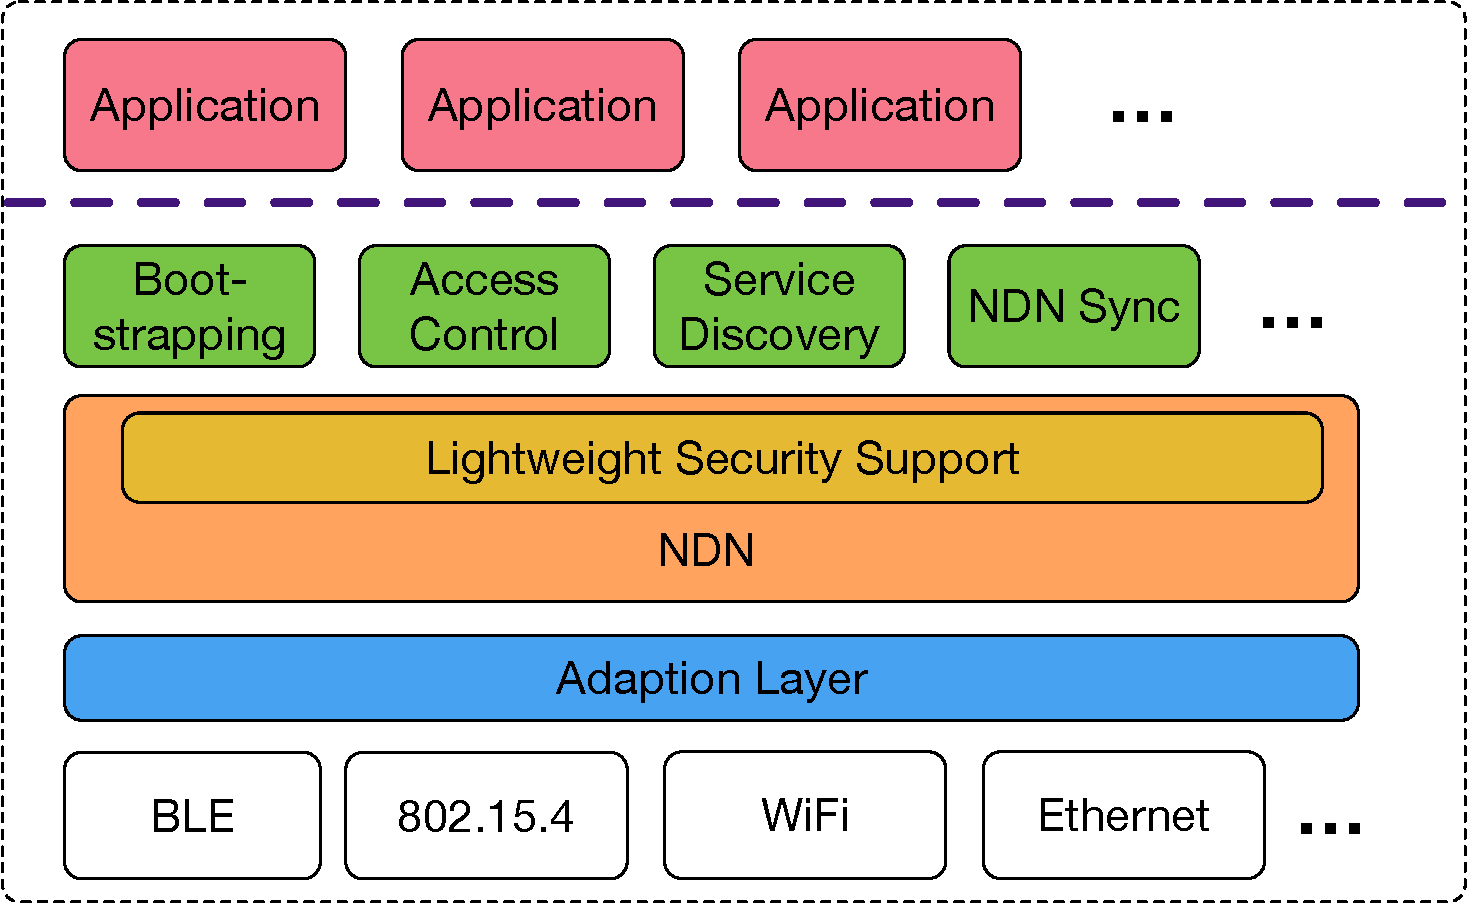
\includegraphics[width=0.4\textwidth]{figures/iot-framework}
	\caption{NDNoT Framework}
	\vspace{-0.2cm}
	\label{fig:framework}
\end{figure}

In this section, we provide a top-down view of the framework and explain how each module works.
%Basically, new coming device should bootstrap first in local NDN, fetching its certificate to explore further services in this scenario. After proper bootstrap and configuration of available services, device will be permitted to exchange data in local NDN. Schematized trust will also be assigned by domain controller to guarantee secure IoT networking.  

\subsection{Bootstrapping}

The bootstrapping module provides applications an automatic way of bootstrapping, which includes both \emph{security} bootstrapping and \emph{network} bootstrapping. 
This module is strictly required for new added devices to
\begin{enumerate*} [label=(\roman*)]
	\item communicate with other IoT devices,
	and
	\item build a trust relationship with the local IoT system and sign/verify NDN Data packets.
\end{enumerate*}

Based on a pre-shared secret (e.g., by scanning a QR code), the security bootstrapping enables an IoT device/application to
\begin{enumerate*} [label=(\roman*)]
	\item install the certificate of the controller as a trust anchor
	and
	\item obtain a certified name linked to a certificate signed by the controller.
\end{enumerate*}
The network bootstrapping step automatically configures the NDN forwarder with the node's available network interfaces (e.g., Bluetooth, BLE, Wi-Fi, IEEE 802.15.4) and learns the name prefix of the connected IoT system.
The NDNoT framework also allows applications to specify which underlying link-layer protocol to use for different communication scenarios.
% Zhiyi, do we really need network bootstrap exists as a independent part? Perhaps this functionality can be included in service discovery. First we need to know the prefixes of BLE, WiFi services and then get their info configured in lightweight nfd.

A new device who want to join the network should have at least one pair of bootstrap key. At the beginning of bootstrap, the 
new coming device should broadcast a interest started with /ndn/sign-on, appended with the digest of BKpub, and a Diffie Hellman key bits.
In this part, considering the time limtation of bootstrap, we use four smaller bits size Diffie Hellman, 64bits for each part, to assembly 
a token to guarantee the security. Although this break down in key bits size will impair the strength of cryptographic operation, given that IoT 
devices, generally have lifetime shorter than ten years, this tradeoff is reasonable. 

\begin{figure}[h]
	\vspace{-0.1cm}
	\centering
	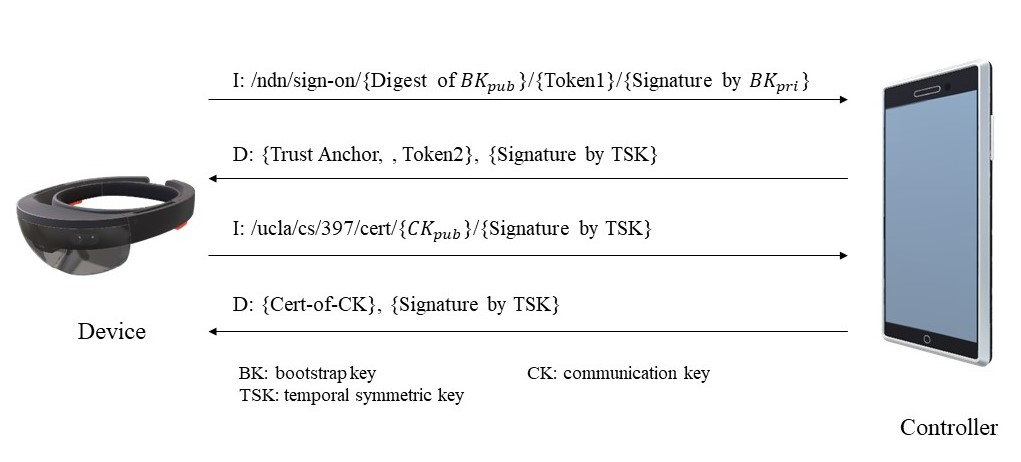
\includegraphics[width=0.45\textwidth]{figures/bootstrap}
	\caption{NDNoT Bootstrap}
	\vspace{-0.1cm}
	\label{fig:bootstrap}
\end{figure}

Device signs this Diffie Hellman key bits included interest with BKpri and send this packet to its IEEE 802.15.4 interface. When controller receives this bootstrap request, it
verify the signature with BKpub fetched from pre-shared secret, and then decide whether to process this request. If the signature is valid,
digest of BKpub in the interest will be extracted, going into a comparation process with the list of pre-shared BKpub keys, proving request
sender has BKpub key. Going through above two verification processes, the request sending device can be trusted by bootstrap controller.
Controller will then send back a bootstrap response, containing the a hash segment, indicating controller hold the BKpub before the bootstrap process, 
an anchor certificate, and four Diffie Hellman key bits parts. This data packet is signed by controller's anchor key. 

After installing the anchor certificate, two sides in bootstrap reach an agreement of trust. On this basis, device can obtain home prefix from 
anchor certificate, and express a certificate interest under the namespace /{home prefix}/cert, signed by Diffie Hellman derived symmetric key.
Certificate request expects an anchor signed certificate from controller, inside which contains a identity allocated from bootstrap controller. 

Basically, an anchor signed certificate is the end of bootstrap, device can extract home prefix and anchor cert from the second round response. 
However, a device who may need several identities to completely utilize its functionalities should bootstrap many times, each time applying for 
one certificate for one identity. 

\subsection{Service Discovery}

The service discovery module helps applications find available services in the local IoT network and also to advertise their own services to other nodes.
Running over NDN, the service discovery is implemented by prefix discovery and prefix registration.
Unlike the service discovery solutions in TCP/IP networks which are based on a (distributed) database query,
NDNoT utilizes NDN's naming convention and the use of application names at the \emph{network layer} to facilitate the discovery/advertisement process.

To start service discovery, the device must be bootstrapped first to obtain the assigned identity name and communication certificate inside the network.
This dependency is guaranteed by system design. three steps are required to begin service discoery. 
\begin{enumerate*} [label=(\roman*)]
	\item device obtains identity and certificate from holder process,
	and
	\item user provides served prefixed in this network.
\end{enumerate*}

After the pre-processes, prefixes are aggregated to several service names, and device will periodically broadcast this service names 
along with identity name obtained from bootstrap distributed certificate, under the namespace {home prefix}/servicediscovery
(e.g., /ucla/cs/397/servicediscovery/sensor1/servicelist/readStatus). The time interval between two broadcast can
be defined users, or set by default. To avoid communication overhead in constrained devices network, a longer interval is preferred, for nodes in
home network scenario being comparatively stationary and stable.  

Other than periodically broadcast interest to notify neighbours the available identity and service names, discovery process also involve a procedure 
to listen other broadcast interest under the namespace {home prefix}/servicediscovery, collecting available identitys and service names around.

\begin{figure}[h]
	\vspace{-0.1cm}
	\centering
	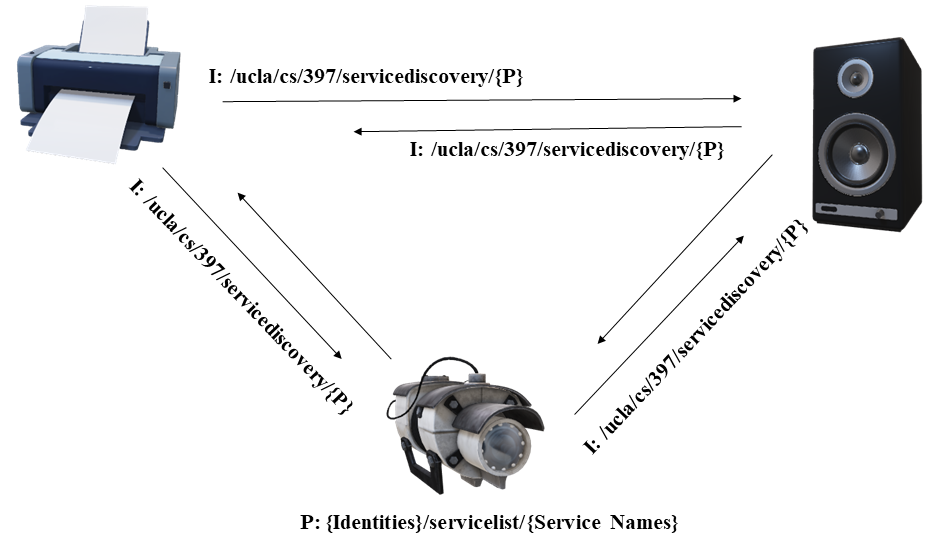
\includegraphics[width=0.45\textwidth]{figures/service-discovery}
	\caption{NDNoT Service Discovery Broadcast}
	\vspace{-0.1cm}
	\label{fig:servicediscovery-broadcast}
\end{figure}

When one want to know more about available services, beyond basic information. It can express a unicast query, which carry specific identity name and service name, 
to device who serve certain prefixes, to ask detailed naming convnetion or parameters needed to apply for this service. An example interest can be 
/ucla/cs/397/sensor0001/query/readStatus, means a bootstrapped device quering device sensor0001 the detail information of service "readStatus". After this query, 
a metadata is expected to come back from target identity.

\begin{figure}[h]
	\vspace{-0.1cm}
	\centering
	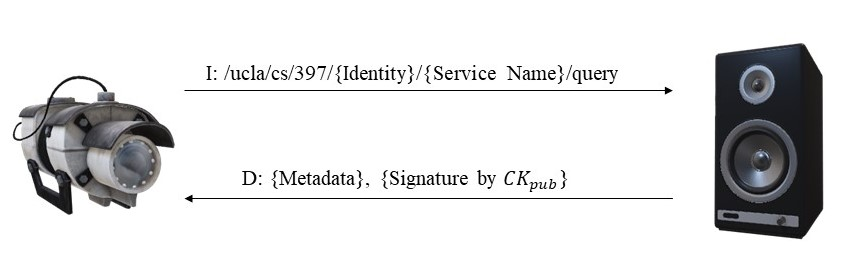
\includegraphics[width=0.45\textwidth]{figures/service-discovery-query}
	\caption{NDNoT Service Discovery Query}
	\vspace{-0.1cm}
	\label{fig:servicediscovery-query}
\end{figure}

In IoT context, an important factor can't be ignored is energy consumption. constrained devices prohibit energy expensive operation, like RF communication, 
from always online. Therefore, devices need to be in sleep mode from time to time, introducing a challenge of delicately tunning all devices awake in same time slot.
However, the synchronization issue is beyond our discussion for now. 

\subsection{Access control}
IoT devices like smart home cameras and door locks require high data confidentiality and strict access control, which are supported by NDNoT's access control module.
Instead of storing the access keys in remote cloud servers, NDNoT provides localized access control, allowing the local user (e.g., home owner) to have complete control of the data produced and consumed by the IoT system.
By naming both digital keys and data, NDNoT automates the key distribution process of the access control scheme, thus minimizing manual configuration.
NDNoT on RIOT OS provide identities based access control and prefixes based access control as two optional modes in our RIOT implementaion. 

\subsubsection{Identities Based Access Control}

A device may serve many prefixes in a home network, each key need update after certain amount of time, leaving key rolling a big issue to developers. Therefore, apply access control on identity, rather than 
certain prefixes is a candidate solution. In this method, a producer first communicate with authentication server, using classic Diffie Hellman key exchange algorithm, to generate a seed for content encryption.
Its access control request interest includes producer's identity name and Diffie Hellman key bits and a ECDSA signature by its communication key. As an optional parameter, a schema of access condition may also 
be appended to the name, indicating to the authentication server what type of consumers can have the decrytion key of the packets from this identity.

\begin{figure}[h]
	\vspace{-0.1cm}
	\centering
	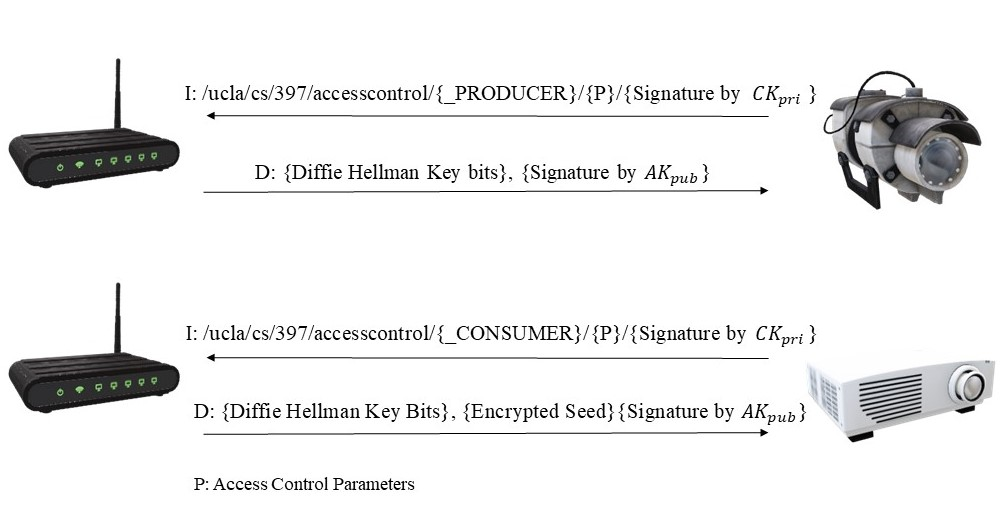
\includegraphics[width=0.45\textwidth]{figures/access-control}
	\caption{NDNoT Access Control}
	\vspace{-0.1cm}
	\label{fig:Access-Control}
\end{figure}

On the access application side, a consumer expresses a access control signed request, which include its identity and identity it want to get access to. This interst also may include an optional parameter in interest 
name to prove the request sender has the right of getting access of certain identities. Successfully verify the signed interest from request sender, the authentication server will firstly search the list of registered 
identity, and check access control schema to decide whether to the applicant have the right to obtain the seed of desired producer identity. After that the authentication server and access applicant will use classic 
Diffie Hellman algorithm to decide the encryption key of transmitting producer's seed on the channel.

\subsubsection{Prefixes Based Access Control}
To devices who need precisely control the access of content, an identity based method is enough. As an alternative solution, we also provide access control on certain producer assigned prefixes. In this schema, producer 
must name specific prefixes.


\subsection{Adaptation Layer}

The adaptation layer abstracts different link-layer protocols and wraps the NDN Interest and Data packets into link-layer frames.
This layer maintains a table indicating which network interface an Interest packet should be forwarded to based on its name.
An application can select different interfaces for different packets simply by tagging NDN packets instead of learning how underlying protocols work and invoking their APIs.
Regarding the implementation, the adaptation layer works as a separate multiplex/demultiplex process and communicates with NDN applications using Inter-Process Communication (IPC) or other equivalent mechanism.

Currently we use IEEE 802.15.4 as link layer protocol in NDNoT on RIOT OS, but the diversity of smart home communication requires us developing more network interfaces, to fit in various scenarioes.

\section{An Application Scenario}

In a classic smart home application scenario, the home owner uses his Android phone or a Linux/macOS laptop as the controller to manage the IoT system.
With NDNoT, each IoT device (e.g., camera, temperature sensor, etc.) trusts the controller and is able to verify signatures generated by other IoT devices, so that the commands or content with fake or untrusted signatures will never be accepted.
Notably, the trust anchor (i.e., the controller certificate) is stored locally on the controller device instead of a remote cloud server.
All devices register their name prefixes for provided services and a device is able to discover the available services under other prefixes by fetching the metadata.
A device records the discovered name prefixes with the corresponding network interfaces (e.g., BLE, 802.15.4) where they are fetched, so that the application simply fetches named content or issues commands without worrying about which network interface to use.
When data privacy is needed, the home owner can configure the access rights for each device/service in the system so that only authorized devices/services can access (i.e., decrypt) the private data.


\section{Current Status and Future Work}

We are currently working on the implementation of NDNoT for boards that work with RIOT and Arduino.
We are adding support for different link-layer network protocols on low-powered devices with limited processing capabilities and, at the same time, optimize the memory and energy efficiency by specializing the implementation for different hardware platforms and link protocols.
We plan to have a live demo of smart home scenarios before October and to release the package by the end of the year.

\bibliographystyle{plain}
\bibliography{ndn}

\end{document}
